%Préambule du document :
\documentclass[12pt, a4paper]{book}
%\usepackage[latin1]{inputenc} 
\usepackage[utf8]{inputenc} % accents
\usepackage{gensymb} % degree symbol ° (\degree)
\usepackage[T1]{fontenc} % | "`pipe"' character
\usepackage{graphicx}
\usepackage{titling}
\usepackage{amssymb} 
\usepackage{minitoc} % chapter's tocs
\usepackage{authblk} % author affiliations
\usepackage{fancyhdr} % modify the headers
\usepackage{tabularx} % tables not larger than A4
\usepackage[table]{xcolor} %colors inside the tables
\usepackage{float}
\usepackage{multicol} % multiple columns in some sections
\usepackage[inner=2cm,outer=2cm]{geometry} %A4 margins
\usepackage{siunitx}
\usepackage[labelfont=bf, margin=0.5cm]{caption} % for figure captions in minipages
\usepackage{hyperref} %link references (toc, citations) inside document
\usepackage{natbib} % to cite with parentheses and plain text et only year if you please...
\usepackage{amsmath}
\usepackage{xcolor}
 \usepackage{fixltx2e} % allows overrightarrow to be in caption
 \MakeRobust{\overrightarrow}




\bibliographystyle{plainnat} % reference style
\renewcommand{\bibname}{References} %Rename "`bibliography"' => "`references"'
\newcommand*{\doi}[1]{\href{https://doi.org/#1}{doi: #1}}

\hypersetup{
    colorlinks,
    citecolor=brown,
    filecolor=green,
    linkcolor=red,
    urlcolor=blue
}
\hypersetup{linktocpage}


\pagestyle{fancy}
\fancyhead{}
\fancyfoot{}
\fancyhead[RO,LE]{\thepage}
\fancyhead[LO]{\leftmark}
\fancyhead[RE]{\rightmark}
\setcounter{tocdepth}{1} % we only want chapters and sections in toc
\setcounter{minitocdepth}{2} %we want sections and subsections in chapters' minitocs

\pretitle{%
  \begin{center}
  
  
\includegraphics[width=17cm]{../Logo_software.png}\\[\bigskipamount]
}
\posttitle{
\\
  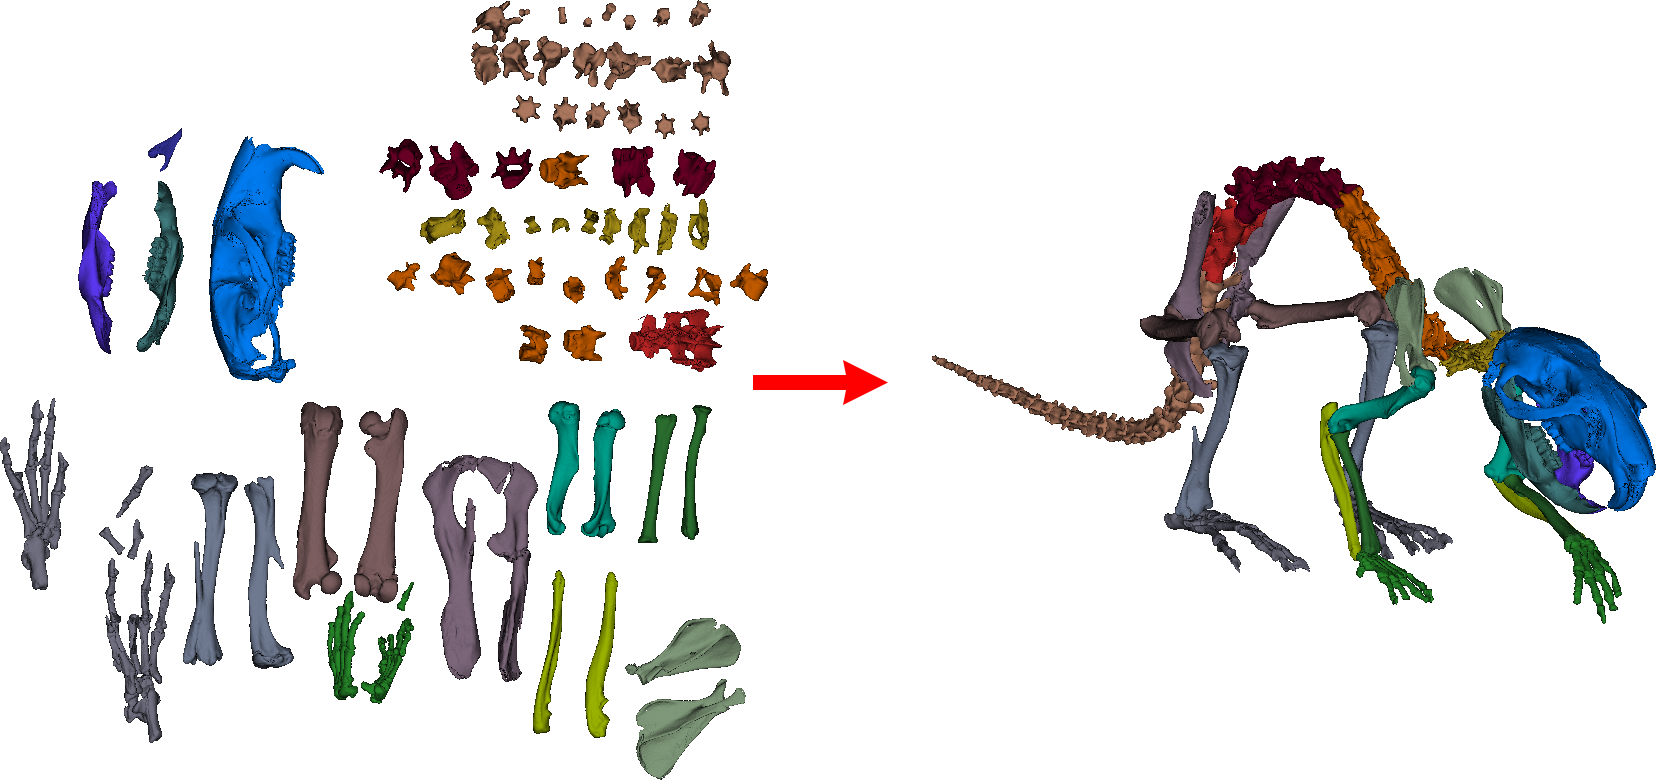
\includegraphics[width=15cm]{tutorial03.png}\\[\bigskipamount]
\end{center}}

%\postdate{
%
\includegraphics[width=15cm]{logo_affiliations.png}
%}

\title{MorphoDig Tutorials\\Tutorial 03: working with many surface objects.}



%\titlepicture[width=13cm]{Logo_software.png}
\author{Renaud LEBRUN}
\affil{Institut des Sciences de l'Evolution, Université de Montpellier, France}
\date{\today} 

\def\chaptername{Tutorial}
\setcounter{chapter}{3}
%Corps du document :
\begin{document}

\dominitoc	

\maketitle

\faketableofcontents
%\tableofcontents

%\chapter{Working with many surface objects}
\addstarredchapter{Working with many surface objects}

\markboth{Tutorial 03: Working with many surface objects}{}

\minitoc 
Tutorial 03 includes:
\begin{itemize}
\item A series of 74 .vtk surface files, each representing a bone belonging to \textit{Canariomys bravoi}
\item Two series of 74 .pos files (to orientate and position each bone)
\item Two .ntw (project) files. The first one to open each bone in initial orientation/position. The second one to opean each bone in anatomical orientation.
\item One .ori (orientation helper labels) file 
\item The present .pdf document
\end{itemize}

Before using this tutorial, please download and read MorphoDig User Guide.


\section{About the present reconstruction}
\subsection{About the specimens}
The present three-dimensional reconstruction of the skeleton of the giant rat of Tenerife (Canary
Islands, Spain) was obtained by computerized microtomography reconstruction. Two distinct specimens
were used in this reconstruction, TFMCV872 and TFMCV873 (Museo de la Naturaleza y el
Hombre, Santa Cruz). TFMCVF872 is an almost complete but disarticulated skeleton of \textit{C. bravoi}. As
mandibles and skull of this specimen were not well preserved, a complete cranium of \textit{C. bravoi} (TFMCVF873)
was added to this reconstruction. The reconstruction of this fossil was published by \citet{Michaux2012} and the 3D model was subsequently disseminated  in MorphoMuseuM \citep{MichauxJ2015}.\\


\subsection{Completeness}
Murinae rodents observed by \citet{Owen1853} always possess a total amount of 19 thoraco-lumbar
vertebrae, most often divided in 13 thoracic and 6 lumbar vertebrae (he also observed at least one
specimen of \textit{Rattus norvegicus} possessing 12 thoracic and 7 lumbar vertebrae). This number of 19
thoraco-lumbar vertebrae is observed very often in mammals and is thought to be a plesiomorphic
condition for eutherians and metatherians mammals (for a review, see for instance \citealp{SanchezVillagra2007}). The present fossil of \textit{C. bravoi} exhibits a number of 17 thoraco-lumbar vertebrae, so there is a high probability that 2 vertebrae (either 1 thoracic and 1 lumbar, or 2 lumbars) are missing.
Furthermore, the number of caudal vertebrae in Murinae rodents observed by \citet{Owen1853} is often greater than the 21 presented in this reconstruction. The present reconstruction of \textit{Canariomys bravoi} does not take into account these potentially missing thoraco-lumbar and caudal vertebrae, and
you may find it sensible to propose new reconstructions of this fossil based on your own observation or Murinae rodents.

\section{Tutorial}
		Download and unzip the files associated to this tutorial.
\subsection{Opening surfaces.}

Download and unzip the 3D files associated to this tutorial. Open MorphoDig.

	You may open the enclosed .vtk surface files (File -> Surface -> Open Surface) or one by one, but as there are 74 surfaces, this is time consuming. MorphoDig offers two faster alternatives:\\
- You may drag and drop all selected files at once in the 3D main window (see Fig. \ref{drag_and_drop}-A p.\pageref{drag_and_drop}).\\
- You may also open all selected files at once when clicking on the "open" (
\includegraphics[scale=0.03]{../images/03/open_data.png}) button inside the main window (or press "CTRL +O").\\

\begin{figure}
  \centering
  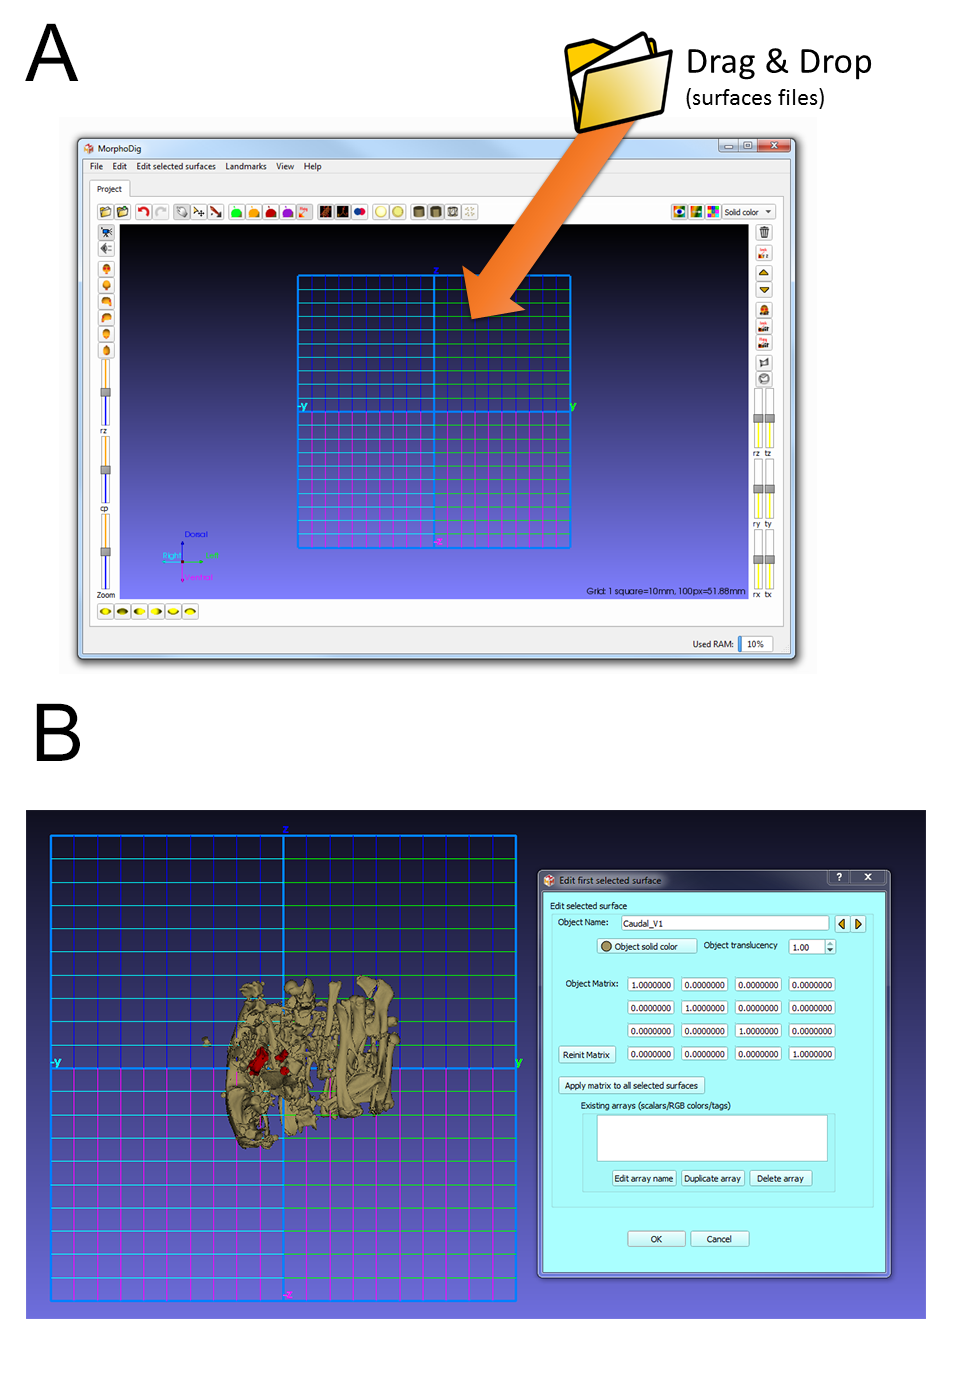
\includegraphics[scale=0.55]{drag_and_drop.png} 
	\caption{Opening many surfaces at once and changing their color.  A: you may drag and drop all 74 surfaces surface at once inside the main 3D window.  B: you may then browse through the 74 opened surfaces via the "Edit first selected surface" window and change the solid color of each bone. }
\label{drag_and_drop}
 
\end{figure}


\subsection{Setting the position of each bone.}

You may interact with selected objects (those which are drawn grey) in different ways (see MorphoDig user guide for further explanations).\\
There are three ways to select one, several or all currently opened surfaces:\\
- \textbf{Selecting surfaces 1 by 1}: press "CTRL +D" to unselect all surfaces and click on "
\includegraphics[scale=0.7]{../images/06/objects/actor_edit.png}": this button opens the "Edit first selected surface" window (see Fig. \ref{drag_and_drop}-B p.\pageref{drag_and_drop}). Then click on 
\includegraphics[scale=0.7]{../images/06/objects/s_right.png} and 
\includegraphics[scale=0.7]{../images/06/objects/s_left.png} to navigate through all opened objects and to select them 1 by 1. That way, you can edit the properties of each of them individually.\\
- \textbf{Selecting surfaces with the mouse}: maintaining the right mouse button pressed while dragging the mouse will draw a selection rectangle. Once the right mouse button has been released, all unselected surfaces laying underneath the selection rectangle will be selected (and all selected surfaces will be unselected).\\
- \textbf{Selecting all surfaces}:\\all opened surfaces can by selected by pressing "CTRL +A" (conversely, all surfaces can be unselected by pressing "CTRL +D")\\




In order to help positioning surfaces in a biologically-relevant manner, 6 predefined camera positions are defined:\\

\includegraphics[scale=0.7]{../images/06/camera/camera_right.png} view object from right side \\

\includegraphics[scale=0.7]{../images/06/camera/camera_left.png} view object from left side\\

\includegraphics[scale=0.7]{../images/06/camera/camera_front.png} view object from front side (default camera position)\\

\includegraphics[scale=0.7]{../images/06/camera/camera_back.png} view object from back side\\

\includegraphics[scale=0.7]{../images/06/camera/camera_above.png} view object from above\\

\includegraphics[scale=0.7]{../images/06/camera/camera_below.png} view object from below\\

In "object interaction mode(
\includegraphics[scale=0.7]{../images/04/move_mode.png})", selected objects can be translated and rotated using the mouse left and middle buttons (in landmark 
\includegraphics[scale=0.7]{../images/04/Landmarks2.png} and camera  
\includegraphics[scale=0.7]{../images/04/camera_mode.png} selection modes, you also need to maintain ``CTRL" button pressed while dragging the left mouse button to achieve rotation and translation of selected objects). Alternatively, you may also use the "yellow sliders" located on the right side of the 3D main window to accomplish rotation and translation of selected objects. Rotation is achieved around the global center of mass of all currently selected objects, which is convenient to rotate groups of bones (ex: all bones belonging a given anatomical unit such as the limbs, the head, the tail etc.) For instance, if you have managed to position the bones belonging to the right
forelimb of \textit{Canariomys bravoi} in anatomical connection after displacing each bone one by one, in a second time, you may select all these bones and displace/rotate the whole forelimb in relation to the other parts of the reconstruction.\\

This tutorial contains two series of 74 .pos files. You may for instance change the position of a selected object by loading a .pos file (File -> Open Position -> Open Position for selected surfaces). For a given bone, you may choose any of the available .pos files, but this only makes sense to choose one of the two related to the currently selected bone. In this tutorial, the .pos files are named the following way:  \textcolor{red}{Bone\_name}\_\textcolor{green}{initial\_position}.pos
or \textcolor{red}{Bone\_name}\_\textcolor{green}{anatomical\_position}.pos.

\subsection{Renaming surfaces}
In some cases, you may need to change the name of some surfaces. For instance, you may disagree with our interpretation of which vertebra is the last thoracic one, and which is the first lumbar one. To change the name of one bone, select one (and only one) surface, click on "
\includegraphics[scale=0.7]{../images/06/objects/actor_edit.png}" to open the "Edit first selected surface" window (see Fig. \ref{drag_and_drop}-B p.\pageref{drag_and_drop}). Then change the "Object Name" field.

\subsection{Projects: save/load the 74 bones and associated properties}
\subsubsection{Saving the project}
Saving a "project" makes it possible to save all opened selected objects at once. In the preceding steps, you may have spent time to change the color and position of each of the 74 surface objects, and saving a "project" is the best way to save your work in a single step. 
To save all opened objects, do the following sequence of actions:\\
1) press "CTRL + A" to select all opened surfaces\\
2) click on "File->Project->Save Project" or on the button "save project" (
\includegraphics[scale=0.03]{../images/03/save_data.png})  inside the main window.\\
3) choose the desired options in the "Save Project" window (see Fig. \ref{save_project_file} p.\pageref{save_project_file} and the User Guide for further details regarding the available options)
\begin{figure}
  \centering  
 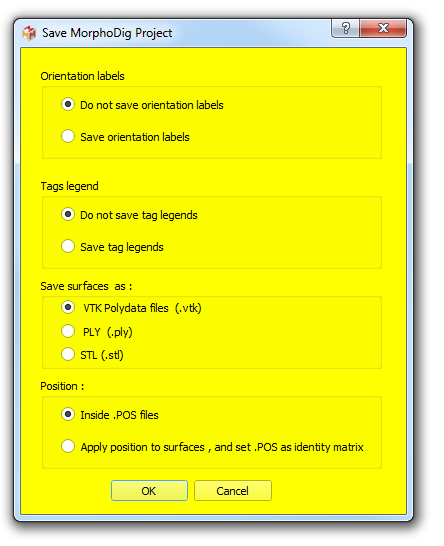
\includegraphics[scale=0.5]{../images/07/project/save_ntw.png}
 \captionof{figure}{Save project window.}
\label{save_project_file}
\end{figure}

The advantage of working with projects is that all involved objects and their properties (surfaces, landmarks, positions etc.) can be reloaded later all at once (and not 1 by 1). 

\subsubsection{Opening projects}
This tutorial contains 2 project (.ntw) files. To open one of them, first delete all opened objects (press "CTRL+A", then press "Del"). Then open one of the two available project files (File -> Project -> Open Project). Choose either "initial\_position.ntw" or "anatomical\_position.
ntw". Once loaded, the 74 surface file objects are opened, are given a position and a color.\\
When
opening "initial\_position.ntw", each bone is given the position described in the file \textcolor{red}{Bone\_name}\_\textcolor{green}{initial\_position}.pos.\\
When opening "anatomical\_position.ntw", each bone is given the position contained in the file \textcolor{red}{Bone\_name}\_\textcolor{green}{anatomical\_position}.pos. The color associated to each bone is defined in the chosen .ntw file. Note that all newly opened surfaces are unselected.

\subsection{\textit{Canariomys} .ori file}
The present tutorial contains a .ori file, which contains orientation labels for the coordinate system
orientation helper. You can load this file the enclosed .ori file ("File->Orientation helper labels -> Open Orientation labels", then select
"Canariomys.ori"). Once loaded, the system coordinate orientation helper will show the following
labels :\\
+z axis : dorsal\\
-z axis : ventral\\
+y axis : left\\
-y axis : right\\
+x axis : proximal\\
-x axis : distal\\
You may set your own orientation axis labels with the "Edit orientation labels" window (Edit-> Edit orientation labels)

\subsection{Acknowledgements}
Iam grateful to María Esther Martín González, curator of the Museo de la Naturaleza y el Hombre,
Santa Cruz, for her enthusiasm regarding the diffusion of the present tutorial. I thank Franck Guy
(formerly IPHEP lab, now PALEVOPRIM), who performed the CT scan of TFMCV872, and the MRI imaging platform for the access to
imaging facilities. The present reconstruction was initiated by Mikael Antocio during the academic
year 2010–2011, at the Paleontology Department, University of Montpellier. Thanks to Lionel Hautier
(ISEM) for his helpful expertise regarding mammalian vertebral anatomy. 

%\nocite{*}   % All bibliography items appear without citation in the text

%\cleardoublepage
%\phantomsection

\addcontentsline{toc}{section}{References}
%\section{References}
 \bibliography{References}		
\end{document} 

